\documentclass[serif,mathserif]{beamer}
\usepackage{etex}
\usepackage{amsmath, amsfonts, epsfig, xspace}
\usepackage{algorithm,algorithmic}
\usepackage{pstricks,pst-node}
\usepackage{multimedia}
\usepackage[normal,tight,center]{subfigure}
\setlength{\subfigcapskip}{-.5em}
\usepackage{beamerthemesplit}
\usetheme{lankton-keynote}
\usepackage{graphicx,color}
% remove caption of figure
\usepackage[labelformat=empty]{caption}

\usepackage[none]{hyphenat} % hyphenation is ugly in slides
\usepackage{parskip}

\usepackage{relsize} % \smaller to change size

\usepackage{tikz}
\usetikzlibrary{calc}

\usetikzlibrary{arrows}

\newcommand{\TikzDraw}[2][]{
  \begin{tikzpicture}[overlay, remember picture, shift={(current page.center)}, #1]
    #2
  \end{tikzpicture}
}

\newcommand{\gridlines}{
  \TikzDraw{
    \draw[help lines,xstep=.2,ystep=.2,red!20] (current page.south west) grid (current page.north east);
    \draw[help lines,xstep=1,ystep=1,red] (current page.south west) grid (current page.north east);
    \foreach \x in {-15,-14,...,15} {
      \node [anchor=north, red] at (\x,0) {\tiny \x};
      \node [anchor=east,red] at (0,\x) {\tiny \x};
    }
  }
}

\newcommand{\DrawOnImg}[3][]
{
  \begin{tikzpicture}
    \node[anchor=south west,inner sep=0] (image) at (0,0){
      #2
    };
    \begin{scope}[x={(image.south east)},y={(image.north west)}]
      \ifthenelse{\equal{#1}{grid}}
                 {\draw[color=blue, style=dashed] (0,0) grid[xstep=.1, ystep=.1] (1.0001,1.0001);}
                 {}
                 #3
    \end{scope}
  \end{tikzpicture}
}


\newcommand{\BOLD}[1]{\mathbf{#1}}
\newcommand{\BOLDG}[1]{\boldsymbol{#1}}
\newcommand{\PDIF}[2]{\frac{\partial #1}{\partial #2}}
\newcommand{\TODO}[1]{\textcolor{red}{#1}}
\newcommand{\TODOB}[1]{\textcolor{blue}{#1}}
\newcommand{\TODOG}[1]{\textcolor{green!50!black}{#1}}
\newcommand{\argmin}{\operatornamewithlimits{arg\min}}
\DeclareMathOperator{\tr}{tr}
\DeclareMathOperator{\cond}{cond}
\DeclareMathOperator{\ST}{s.t.}
\DeclareMathOperator{\diag}{diag}

\author[Jiong Chen]{Jiong Chen}

\title[\hspace{2em}\insertframenumber/\inserttotalframenumber]{A Brief on Deep Learning}

\date{December 30, 2016}

% \institute{Zhejiang University}

\begin{document}

\maketitle

\begin{frame}
  \frametitle{Simple Review on Regression}
  \begin{itemize}
    \visible<1-> {\item Training data $\{(y_i, x_i)\}\rightarrow y = f(x)$}
    \visible<2-> {\item Linear regression
    \begin{equation*}
      \min_{w} \sum_{i=1}^N \|y_i - w^Tx_i\|^2
    \end{equation*}
    }
    \visible<3-> {\item Nonlinear regression method
    \begin{equation*}
      \min_{w} \sum_{i=1}^N \|y_i - w^Th(x_i) \|^2
    \end{equation*}
    }
    \visible<4-> {\item Kernel method
    \begin{equation*}
      \mathcal{K}(x, x') = <h(x), h(x')>
    \end{equation*}
    }
    %% \begin{equation*}
    %%   \begin{split}
    %%     \beta &=(\BOLD{H}^T\BOLD{H}+\lambda \BOLD{I})^{-1}\BOLD{H}^T\BOLD{y} \\
    %%     & = (\BOLD{H}^T\BOLD{H}+\lambda \BOLD{I})^{-1}\BOLD{H}^T(HH^T+\lambda I)(HH^T+\lambda I)^{-1}\BOLD{y} \\
    %%     & = (\BOLD{H}^T\BOLD{H}+\lambda \BOLD{I})^{-1}(H^TH+\lambda I)H^T(HH^T+\lambda I)^{-1}\BOLD{y} \\
    %%     &=  \BOLD{H}^T(\BOLD{HH}^T+\lambda \BOLD{I})^{-1}\BOLD{y}
    %%   \end{split}
    %% \end{equation*}
  \end{itemize}
  \TikzDraw {
    \visible<2> {\node at (0.4, -0.5) {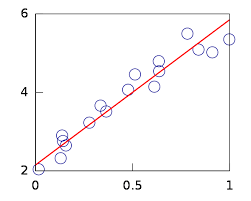
\includegraphics[width=0.3\textwidth]{img/linreg}};}
    \visible<3> {\node at (0.4, -2.5) {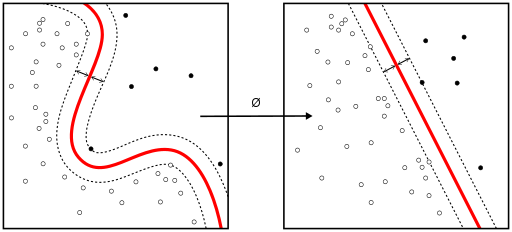
\includegraphics[width=0.4\textwidth]{img/kernelmethod}};}
  }
\end{frame}

\begin{frame}
  \frametitle{Why Deep Learning}
  \begin{itemize}
  \item Limitation of these regression methods
    \begin{itemize}
    \item Linear regression: most procedure is nonlinear
    \item Kernel method: not generalized well far from the training examples
    \item Hand design features require a large amount of engineering skill and domain expertise 
    \end{itemize}
  \item Is there a general-purpose learning procedure that can automatically
    learn good features?
  \end{itemize}
\end{frame}

\begin{frame}
  \frametitle{Neural Networks}
  \TikzDraw {
    \node at (-1.6, 0) { \parbox[]{0.8\textwidth} {
        \begin{itemize}
          \visible<1-> {\item Structure: stacked layers of neurons}
          \visible<2-> {\item Mathematical formulation
          \begin{equation*}
            \begin{split}
              &Z_m = \sigma(\alpha_{m0}+\alpha_m^TX), \\
              &T_k = \beta_{k0} + \beta_k^TZ, \\
              &f_k(X) = g_k(T)
            \end{split}
          \end{equation*}
        \item Loss function
          \begin{equation*}
            \begin{split}
              &R(w) = \sum_{k=1}^K \|y_k - f_k(x) \|^2~~(\text{fitting})\\
              &R(w) = \sum_{k=1}^K y_k\log f_k(x)~~(\text{classification})
            \end{split}
          \end{equation*}
          }
        \end{itemize}
      }
    };
    \node at (3.6, 0.5) {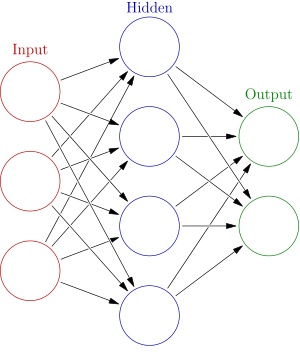
\includegraphics[width=0.4\textwidth]{img/nnet}};
    \node at (1.9, 1.8) {\textcolor{red}{$X_1$}};
    \node at (1.9, 0.5) {\textcolor{red}{$X_2$}};
    \node at (1.9, -0.8) {\textcolor{red}{$X_3$}};
    \node at (3.6, 2.4) {\textcolor{blue}{$Z_1$}};
    \node at (3.6, 1.1) {\textcolor{blue}{$Z_2$}};
    \node at (3.6, -0.1) {\textcolor{blue}{$Z_3$}};
    \node at (3.6, -1.4) {\textcolor{blue}{$Z_4$}};
    \node at (5.35, 1.1) {\textcolor{green}{$T_1$}};
    \node at (5.35, -0.1) {\textcolor{green}{$T_2$}};
    \node at (2.6, 0.5) {\textcolor{orange}{$\BOLDG{\alpha}$}};
    \node at (4.5, 0.5) {\textcolor{orange}{$\BOLDG{\beta}$}};
  }
  %\gridlines
\end{frame}

\begin{frame}
  \frametitle{Activation Functions}
  \begin{itemize}
  \item Sigmoid
    \begin{equation*}
      \begin{split}
        \sigma(x) &= \frac{1}{1+e^{-x}} \\
        \sigma'(x) &= \sigma(x)(1-\sigma(x))
      \end{split}
    \end{equation*}
  \item TanH
    \begin{equation*}
      \begin{split}
        \sigma(x) &= \frac{1-e^{-2x}}{1+e^{2x}} \\
        \sigma'(x) &= 1-\sigma(x)^2
      \end{split}
    \end{equation*}
  \end{itemize}
  \TikzDraw {
    \node at (4.2, 1.5) {\includegraphics[width=0.3\textwidth]{img/sigmoid}};
    \node at (4.2, -2) {\includegraphics[width=0.3\textwidth]{img/tanh}};
  }
\end{frame}

\begin{frame}
  \frametitle{Training}
  \TikzDraw {
    \node at (-3.2, 0) {\parbox[]{0.5\textwidth} {
        \begin{itemize}
          \visible<1-> {\item How to compute gradient?}
          \visible<2-> {\item \textcolor{red}{\textit{Back Propagation}}}
          \visible<3-> {
            \begin{equation*}
              \boxed{
                \begin{split}
                  &z_l = W_{lk}y_k \Rightarrow \\
                  &\PDIF{E}{W_{lk}}=\PDIF{E}{z_l}\PDIF{z_l}{W_{lk}}= \PDIF{E_z}{z_l}y_k\\
                  &\PDIF{E}{y_k} = \PDIF{E}{z_l}\PDIF{z_l}{y_k} = \PDIF{E}{z_l}W_{lk}
                \end{split}
              }
            \end{equation*}
          }
          \visible<4-> {
          \item Optimization (forward + backward)
            \begin{itemize}
            \item LBFGS
            \item SGD
            \item Adaptive gradient
            \item ...
            \end{itemize}
          }
        \end{itemize}
      }
    };
    \visible<2-> {\node at (3.2, 0) {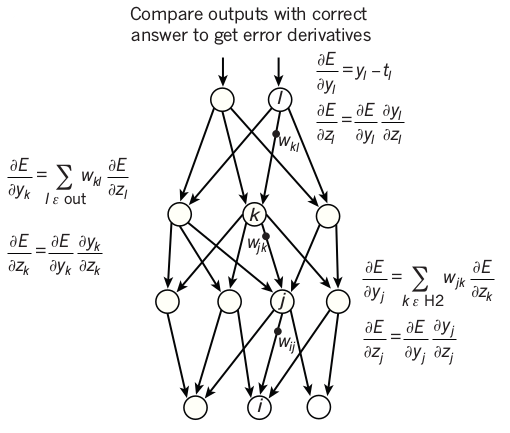
\includegraphics[width=0.6\textwidth]{img/BP}};}
    \visible<3-> {
      \draw[red, thick, dashed] (2.1, 0.18) rectangle (4.2, 1.4);
    }
    \visible<1> {\node at (3.2, 0) {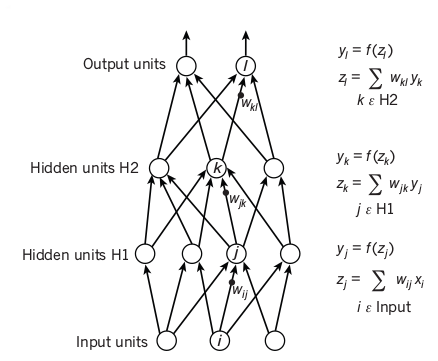
\includegraphics[width=0.55\textwidth]{img/FP}};}
  }
  %\gridlines
\end{frame}

\begin{frame}
  \frametitle{Going Deeper}
  \begin{itemize}
  \item Deep network has more powerful abstraction capability than shallow one
    \pause
  \item However...
    \begin{figure}
      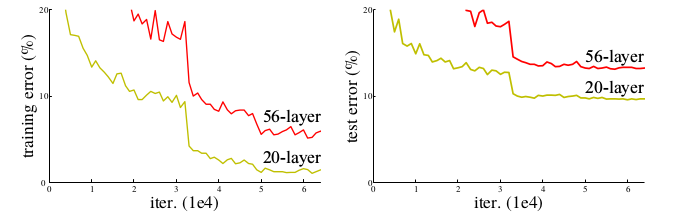
\includegraphics[width=0.8\textwidth]{img/deepdifficulty}
    \end{figure}
  \item Learning better networks is not easy as stacking more layers
  \end{itemize}
\end{frame}

\begin{frame}
  \frametitle{Understanding the difficulty}
  \begin{itemize}
  \item Local minima of high dimensional non-convex optimization 
  \item Degradation problem
    \begin{figure}
      \centering
      \includegraphics[width=0.4\textwidth]{img/sigmoiddiff}
    \end{figure}    
  \end{itemize}
\end{frame}

\begin{frame}
  \frametitle{Efforts on making network deeper}
  \begin{itemize}
  \item Weights initialization
    \begin{itemize}
    \item Unsupervised pre-training
    \item Reducing the dimensionality of data with neural network, 2006
      \begin{figure}
        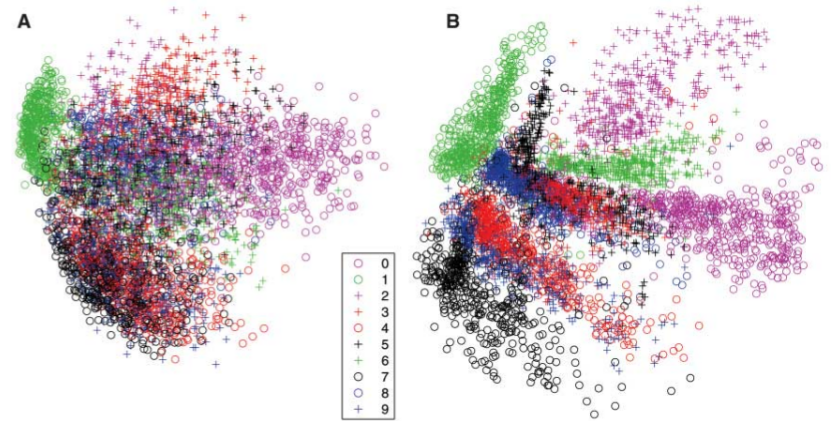
\includegraphics[width=0.6\textwidth]{img/PCAandNN}
      \end{figure}
    \end{itemize}
  \end{itemize}
\end{frame}

\begin{frame}
  \frametitle{Efforts on making network deeper}
  \begin{itemize}
  \item Rectified Linear Unit (ReLU) $\sigma(x) = \max(0, x)$
    \begin{itemize}
    \item Speed
    \item Sparsity
    \item Intensity preserving
      \visible<3-> {\item \emph{``... Can reach their best performance without requiring any unsupervised
          pre-training on purely supervised tasks with large labeled data.''
          ------Deep sparse rectifier neural network, 2011}}
    \end{itemize}
  \end{itemize}
  \TikzDraw {
    \visible<1> {
      \node at (2.5, -.5) {\includegraphics[width=0.5\textwidth]{img/relu}};
    }
    \visible<2> {
      \node at (2.7, -.3) {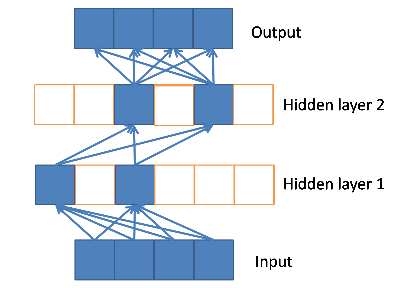
\includegraphics[width=0.4\textwidth]{img/sparseRelu}};
    }
  }
\end{frame}

\begin{frame}
  \frametitle{Efforts on making network deeper}
  \begin{itemize}
  \item Batch normalization (2015)
    \begin{itemize}
    \item Distribution of each layer's input changes during training
    \item BN $\rightarrow$ mean = 0, variance = 1
      \visible<1> {
      \begin{figure}
        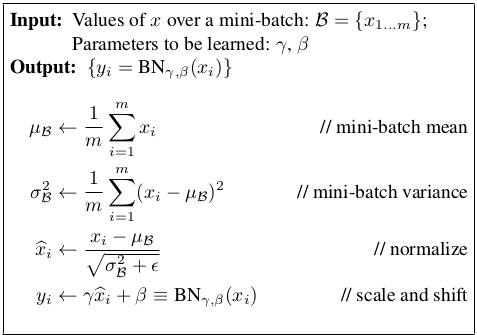
\includegraphics[width=0.5\textwidth]{img/BN}
      \end{figure}
      }
    \end{itemize}
  \end{itemize}
  \TikzDraw {
    \visible<2> {
      \node at (-3, -1) {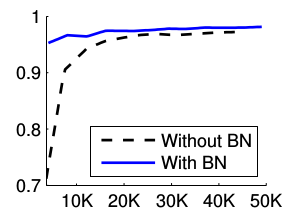
\includegraphics[width=0.4\textwidth]{img/BNmnist}};
      \node at (2.5, -1) {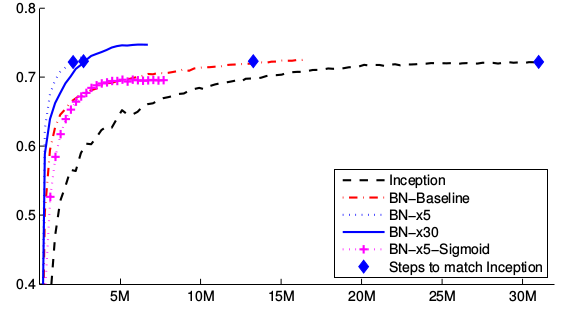
\includegraphics[width=0.55\textwidth]{img/BNimagenet}};
      \node at (-3, -3) {MNIST};
      \node at (2.5, -3) {ImageNet};
    }
  }
\end{frame}

\begin{frame}
  \frametitle{Efforts on making network deeper}
  \TikzDraw {
    \node at (-1.6, 0) {\parbox[]{0.8\textwidth} {
        \begin{itemize}
        \item Residual learning (2016)
          \begin{itemize}
          \item Problem of learning identity mapping
          \item Skip connections (shortcut)
            \begin{figure}
              \centering
              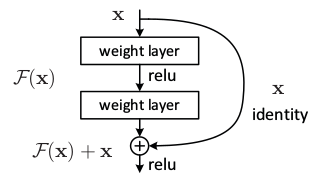
\includegraphics[width=0.4\textwidth]{img/skip}
            \end{figure}
          \item Back propagation
            \begin{equation*}
              \begin{split}
                \PDIF{E}{x_l}& = \PDIF{E}{x_L}\textcolor{blue}{\PDIF{x_L}{x_l}} \\
                &= \PDIF{E}{x_L}\textcolor{blue}{(1+\PDIF{}{x_l}\sum_{i=1}^{L-1}\mathcal{F}(x_i, W_i))}
              \end{split}
            \end{equation*}
          \end{itemize}
        \end{itemize}
    }};
  }
  \TikzDraw {
    \node at (-0.8, 2) {\textcolor{red}{$x_l$}};
    \node at (-0.8, 0.4) {\textcolor{red}{$x_L$}};
    \visible<2-> {\node at (4, -0.2) {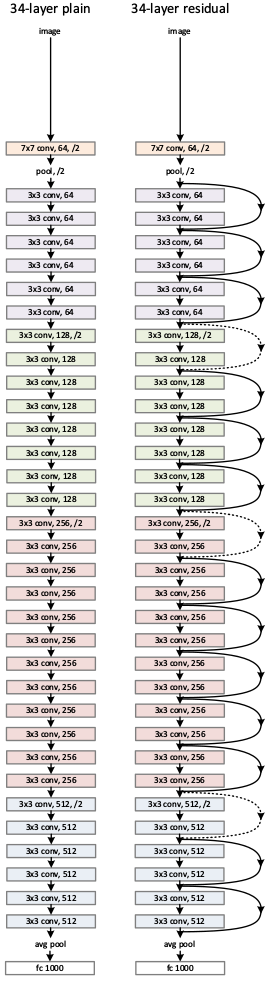
\includegraphics[width=0.2\textwidth]{img/deepres}};}
  }
  %\gridlines
\end{frame}

\begin{frame}
  \frametitle{Generalization: ConvNets}
  \begin{itemize}
    \visible<1-> {\item Designed to process data that come in the form of multiple arrays}
    \visible<2-> {\item Four key ideas: \emph{local connections, shared weights, pooling and use of many layers}}
    \visible<3-> {\item Convolutional layer: detect local feature conjunctions}
    \visible<4-> {\item Pooling layer: merge semantically similar features}
  \end{itemize}
  \TikzDraw {
    \visible<1> {
      \node at (0, -0.5) {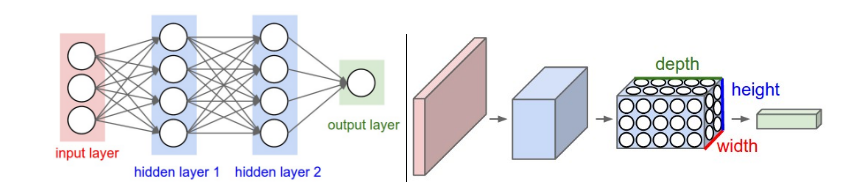
\includegraphics[width=\textwidth]{img/convnet}};
      \draw[red, thick, dashed] (0.95, -1.5) rectangle (2.1, 0);
      \node at (1.5, 0.4) {\scriptsize{\textcolor{red}{3D volumes of neurons}}};
    }
    \visible<3> {
      \node at (-3, -2.5) {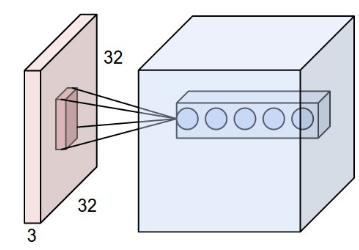
\includegraphics[width=0.3\textwidth]{img/convlayer}};
      \node at (2.6, -2.5) {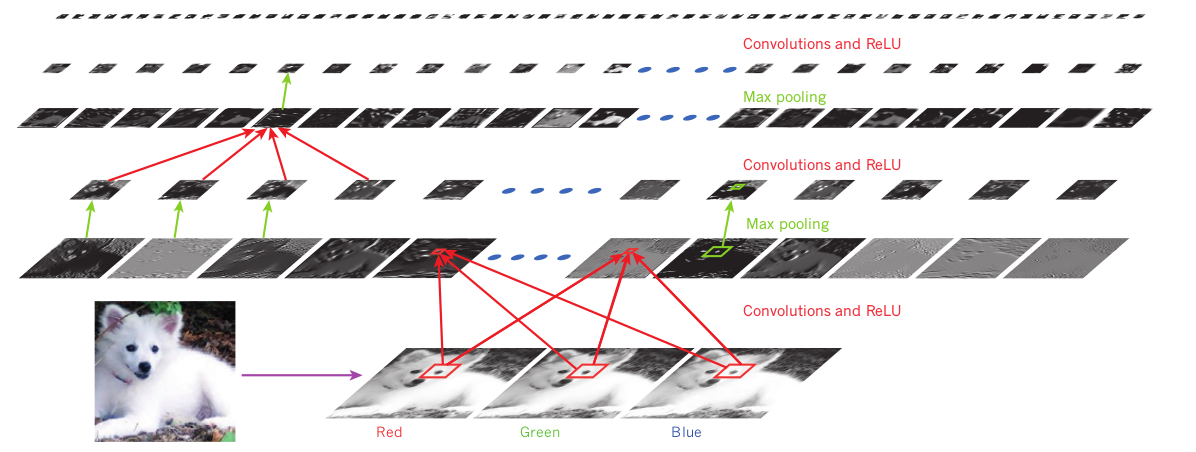
\includegraphics[width=0.65\textwidth]{img/samoyed}};
      \node at (-2.9, -2.64) {\tiny{\textcolor{blue}{$w_1$}}};
      \node at (-2.6, -2.64) {\tiny{\textcolor{blue}{$w_2$}}};
      \node at (-2.3, -2.64) {\tiny{\textcolor{blue}{...}}};
    }
    \visible<4-> {
      \node at (-2, -2.8) {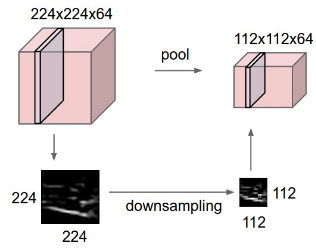
\includegraphics[width=0.3\textwidth]{img/poolinglayer}};
      \node at (2.5, -2.7) {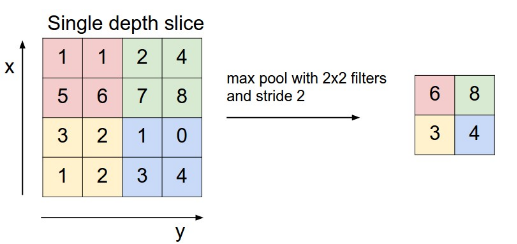
\includegraphics[width=0.4\textwidth]{img/maxpool}};
    }
  }
  %\gridlines
\end{frame}

\begin{frame}
  \frametitle{Generalization: ConvNets}
  \begin{itemize}
  \item ImageNet: 14,197,122 images, 21841 synsets indexed
  \item Large Scale Visual Recognition Challenge (ILSVRC)
    \begin{itemize}
    \item \textbf{\textcolor{red}{AlexNet}}
      \emph{``Imagenet classification with deep convolutional neural networks.'' 2012}
    \item \textbf{\textcolor{red}{VGGNet}}
      \emph{``Very deep convolutional networks for large-scale image recognition.'' 2014}
    \item \textbf{\textcolor{red}{GoogLeNet}}
      \emph{``Going deeper with convolutions.'' 2015.}
    \item \textbf{\textcolor{red}{ResNet}}
      \emph{``Deep residual learning for image recognition.'' 2016}
    \end{itemize}
  \end{itemize}
\end{frame}

\begin{frame}
  \frametitle{Generalization: RNN}
  \begin{itemize}
  \item Recurrent Neural Network: handle sequential input
    \begin{itemize}
    \item maintain `state vector' in hidden layers
    \end{itemize}
  \item Unfolding of the RNN
    \begin{figure}
      \centering
      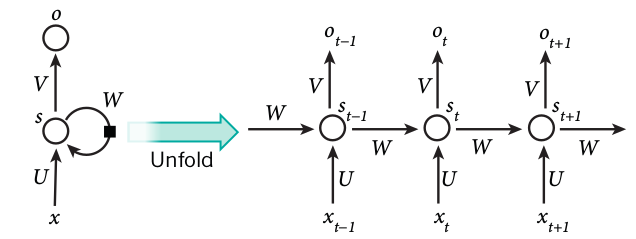
\includegraphics[width=\textwidth]{img/unfolding}
    \end{figure}
  \end{itemize}
\end{frame}

\begin{frame} 
  \TikzDraw {
    \node at (0, 0.5) {\Huge{Thanks!}};
  }
  %\gridlines
\end{frame}


\end{document}
